% Options for packages loaded elsewhere
\PassOptionsToPackage{unicode}{hyperref}
\PassOptionsToPackage{hyphens}{url}
%
\documentclass[
]{article}
\usepackage{lmodern}
\usepackage{amssymb,amsmath}
\usepackage{ifxetex,ifluatex}
\ifnum 0\ifxetex 1\fi\ifluatex 1\fi=0 % if pdftex
  \usepackage[T1]{fontenc}
  \usepackage[utf8]{inputenc}
  \usepackage{textcomp} % provide euro and other symbols
\else % if luatex or xetex
  \usepackage{unicode-math}
  \defaultfontfeatures{Scale=MatchLowercase}
  \defaultfontfeatures[\rmfamily]{Ligatures=TeX,Scale=1}
\fi
% Use upquote if available, for straight quotes in verbatim environments
\IfFileExists{upquote.sty}{\usepackage{upquote}}{}
\IfFileExists{microtype.sty}{% use microtype if available
  \usepackage[]{microtype}
  \UseMicrotypeSet[protrusion]{basicmath} % disable protrusion for tt fonts
}{}
\makeatletter
\@ifundefined{KOMAClassName}{% if non-KOMA class
  \IfFileExists{parskip.sty}{%
    \usepackage{parskip}
  }{% else
    \setlength{\parindent}{0pt}
    \setlength{\parskip}{6pt plus 2pt minus 1pt}}
}{% if KOMA class
  \KOMAoptions{parskip=half}}
\makeatother
\usepackage{xcolor}
\IfFileExists{xurl.sty}{\usepackage{xurl}}{} % add URL line breaks if available
\IfFileExists{bookmark.sty}{\usepackage{bookmark}}{\usepackage{hyperref}}
\hypersetup{
  hidelinks,
  pdfcreator={LaTeX via pandoc}}
\urlstyle{same} % disable monospaced font for URLs
\usepackage[margin=1in]{geometry}
\usepackage{graphicx,grffile}
\makeatletter
\def\maxwidth{\ifdim\Gin@nat@width>\linewidth\linewidth\else\Gin@nat@width\fi}
\def\maxheight{\ifdim\Gin@nat@height>\textheight\textheight\else\Gin@nat@height\fi}
\makeatother
% Scale images if necessary, so that they will not overflow the page
% margins by default, and it is still possible to overwrite the defaults
% using explicit options in \includegraphics[width, height, ...]{}
\setkeys{Gin}{width=\maxwidth,height=\maxheight,keepaspectratio}
% Set default figure placement to htbp
\makeatletter
\def\fps@figure{htbp}
\makeatother
\setlength{\emergencystretch}{3em} % prevent overfull lines
\providecommand{\tightlist}{%
  \setlength{\itemsep}{0pt}\setlength{\parskip}{0pt}}
\setcounter{secnumdepth}{-\maxdimen} % remove section numbering

\title{\includegraphics[width=8in,height=\textheight]{V:/Bello_M/BACKUP/Science Barometer/Codes/OECDwithIDBlogo.JPG}

Science in the face of the COVID-19 crisis}
\author{}
\date{\vspace{-2.5em}}

\begin{document}
\maketitle

\hypertarget{oecd-science-flash-survey-2020}{%
\subsection{OECD Science Flash Survey
2020}\label{oecd-science-flash-survey-2020}}

Experimental results, last updated on 19 October, 2020

This document provides a real-time glance at the initial results from
the new OECD Science Flash Survey 2020. This ``flash'' or ``pulse''
survey was designed and first launched by the OECD Directorate for
Science, Technology and Innovation on an experimental basis in mid-April
2020. Its objective is to provide a timely picture -- i.e.~a pulse
measure -- of the state of science amidst the COVID-19 crisis and report
on society's perceptions about its role and future outlook. Scientific
research and the use of scientific evidence are key aspects of the
global and OECD effort against the pandemic and its economic and social
repercussions. This survey complements the STIP-COVID survey on policy
responses to the crisis.

\hypertarget{methodology-an-experimental-oecd-study}{%
\subsection{\texorpdfstring{\textbf{Methodology -- an experimental OECD
study}}{Methodology -- an experimental OECD study}}\label{methodology-an-experimental-oecd-study}}

This study has been implemented through an online open-link
questionnaire {[}click to participate{]}, inviting scientists or any
other individuals with an interest in science or science policy on the
impact of the COVID-19 crisis from a science perspective. The survey, so
far only available in English, has been initially promoted through the
network of the OECD Committee for Scientific and Technological Policy
and former participants of the 2018 OECD International Survey of
Scientific Authors (ISSA). Given its focus on getting a pulse on the
situation and outlook, the survey design prioritises timeliness and full
anonymity. The survey does not request any information that can identify
the respondents. As a result, results cannot be considered to be
representative of a well-defined population and should be treated with
extreme caution and considered as a complementary view to other
statistical evidence.

\hypertarget{highlights}{%
\subsection{\texorpdfstring{\textbf{Highlights}}{Highlights}}\label{highlights}}

As of 19 October, 2020, over 2600 responses from nearly 100 countries
have been collected. 45\% of responses correspond to individuals that
identify themselves as scientists, with the rest comprising science
policy advisors (20\%), professionals involved in science (15\%),
science communicators (10\%) and individuals carrying out
science-related administrative work (10\%). 70\% of responses indicate a
shift to home working. Nearly 20\% report a shift of the orientation of
their work towards COVID-19-related issues.15\% of responses from
scientists reported a reduction in the intensity of their work, compared
to about 20\% reporting an increase in intensity.

\hypertarget{impact-of-the-covid-19-crisis-on-scientific-research}{%
\section{\texorpdfstring{\textbf{Impact of the COVID-19 crisis on
scientific
research}}{Impact of the COVID-19 crisis on scientific research}}\label{impact-of-the-covid-19-crisis-on-scientific-research}}

Responses indicating a recent experience or expectation of upcoming
changes under each of the following items.

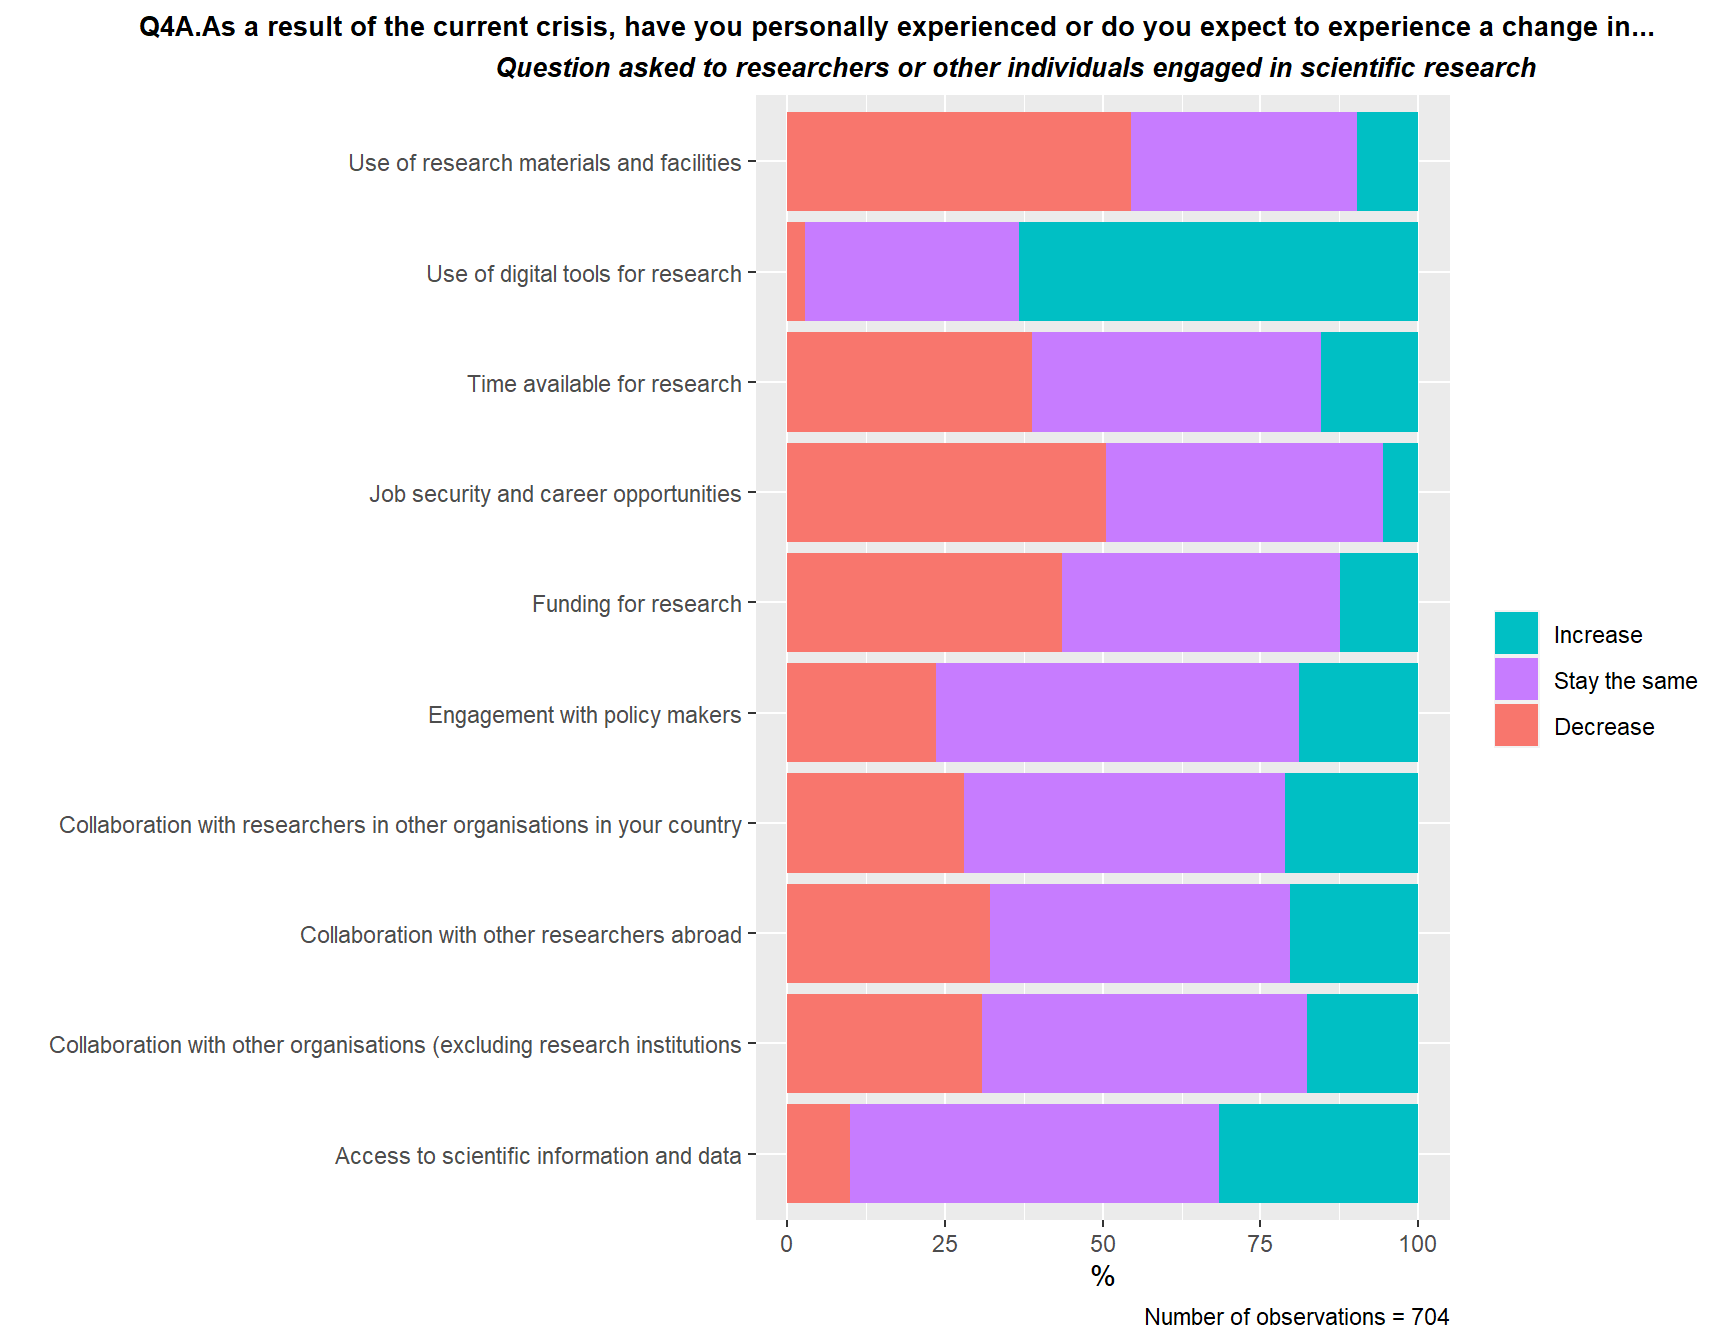
\includegraphics{V:/Bello_M/BACKUP/Science Barometer/Git/2020flashsciencecovid/docs/index_files/figure-latex/plot_corecharts0-1.pdf}

The responses from scientists reveal a negative impact on the use of
research material and facilities, job security and career opportunities,
research funding and time available for research. A minority of
responses expect a change in collaboration and engagement with policy
makers. Collaboration is expected to be slightly negatively impacted.
Scientists' impressions point towards an increased use of digital tools
for research and access to scientific information and data as a
consequence of the current crisis. No large differences are found
between women and men. Yet women point to a stronger decrease in their
time available for research.

\hypertarget{respondents-expectations-about-the-future-of-the-world-of-science}{%
\section{\texorpdfstring{\textbf{Respondents' expectations about the
future of the world of
science}}{Respondents' expectations about the future of the world of science}}\label{respondents-expectations-about-the-future-of-the-world-of-science}}

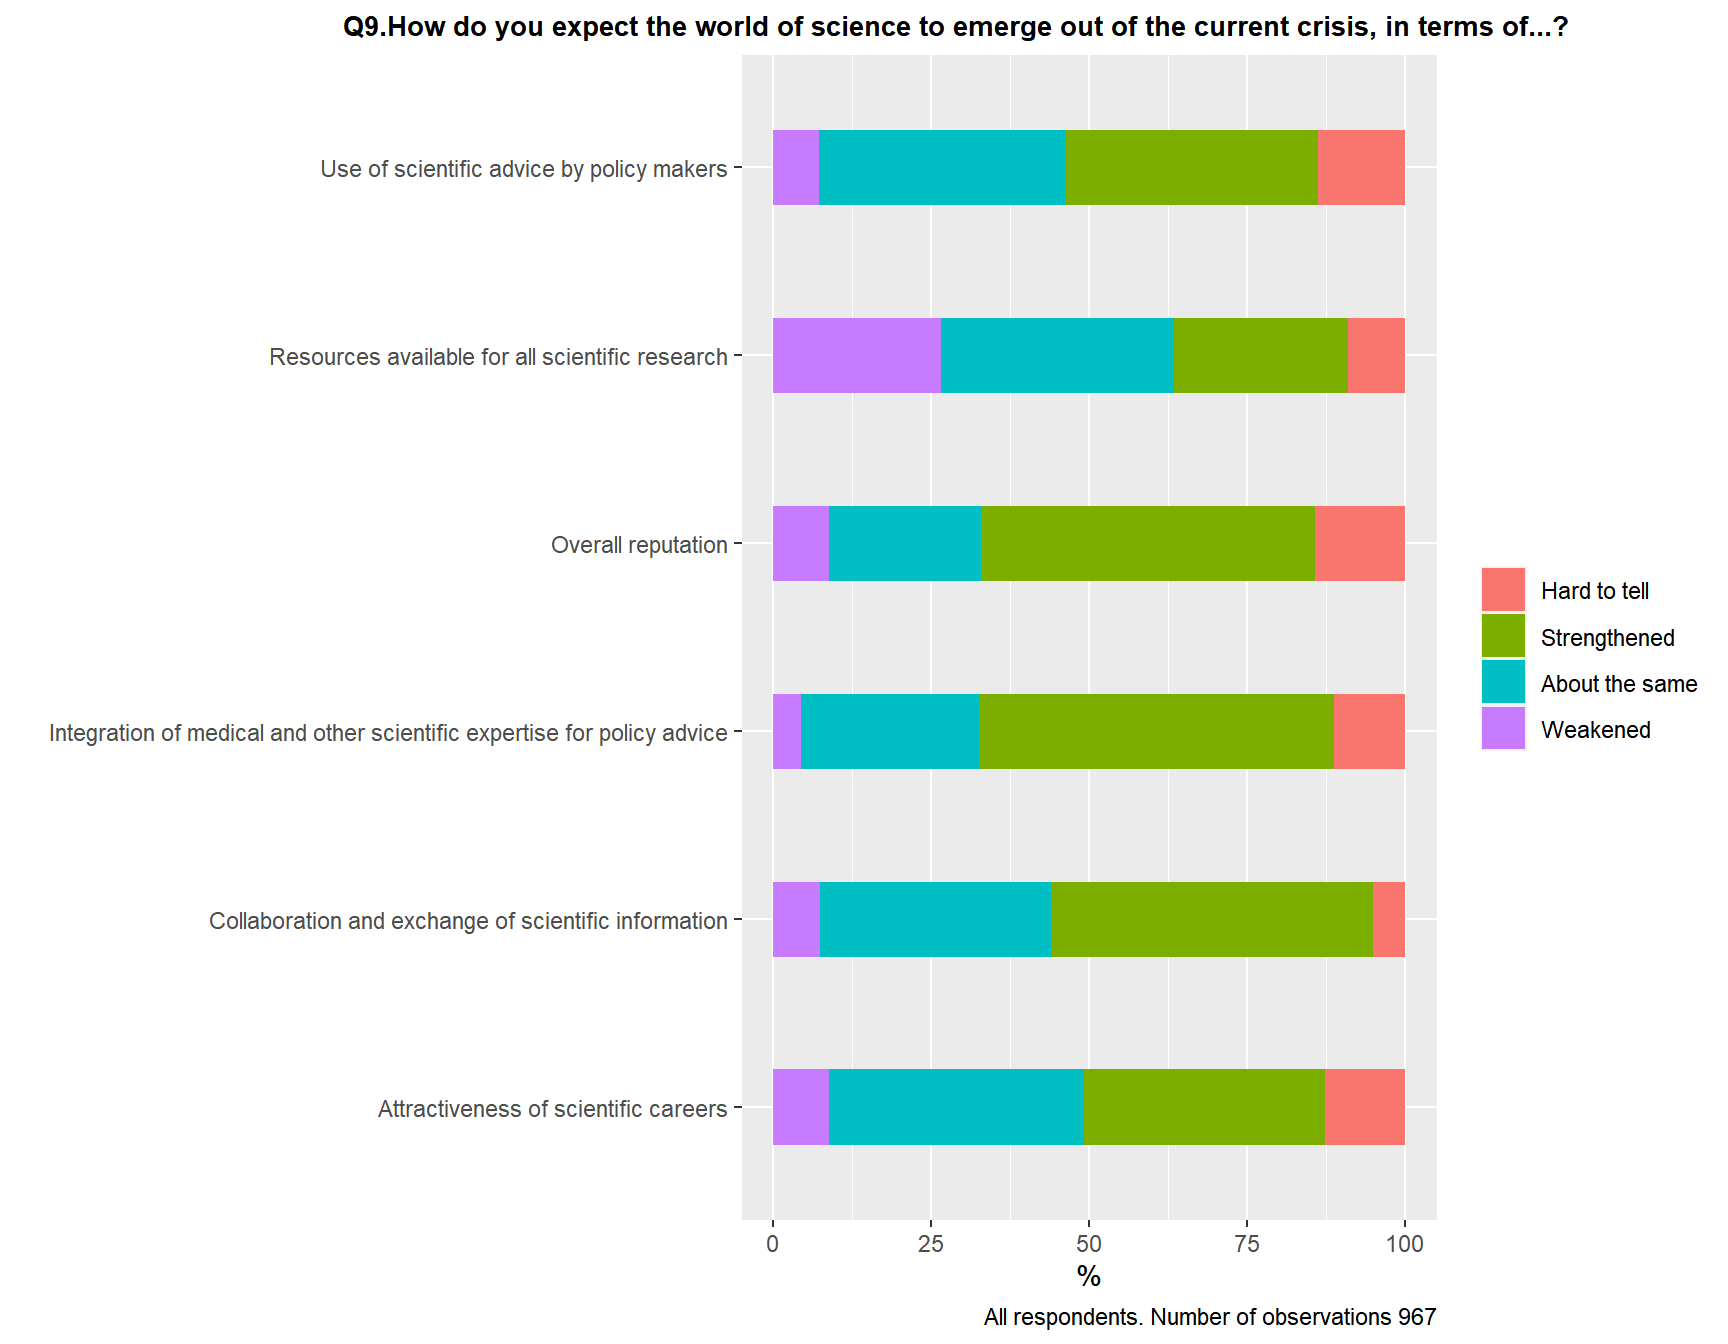
\includegraphics{V:/Bello_M/BACKUP/Science Barometer/Git/2020flashsciencecovid/docs/index_files/figure-latex/plot_corecharts1-1.pdf}

The responses collected thus far are overall positive about the general
prospects for the status of science after the crisis. Respondents expect
science to see its reputation strengthening and foresee a greater use
and integration of different strands of scientific expertise in policy
advice as well as stronger collaboration and exchange of scientific
information. However, respondents are highly uncertain about the overall
resources that will be available for scientific research after the
COVID-19 pandemic.

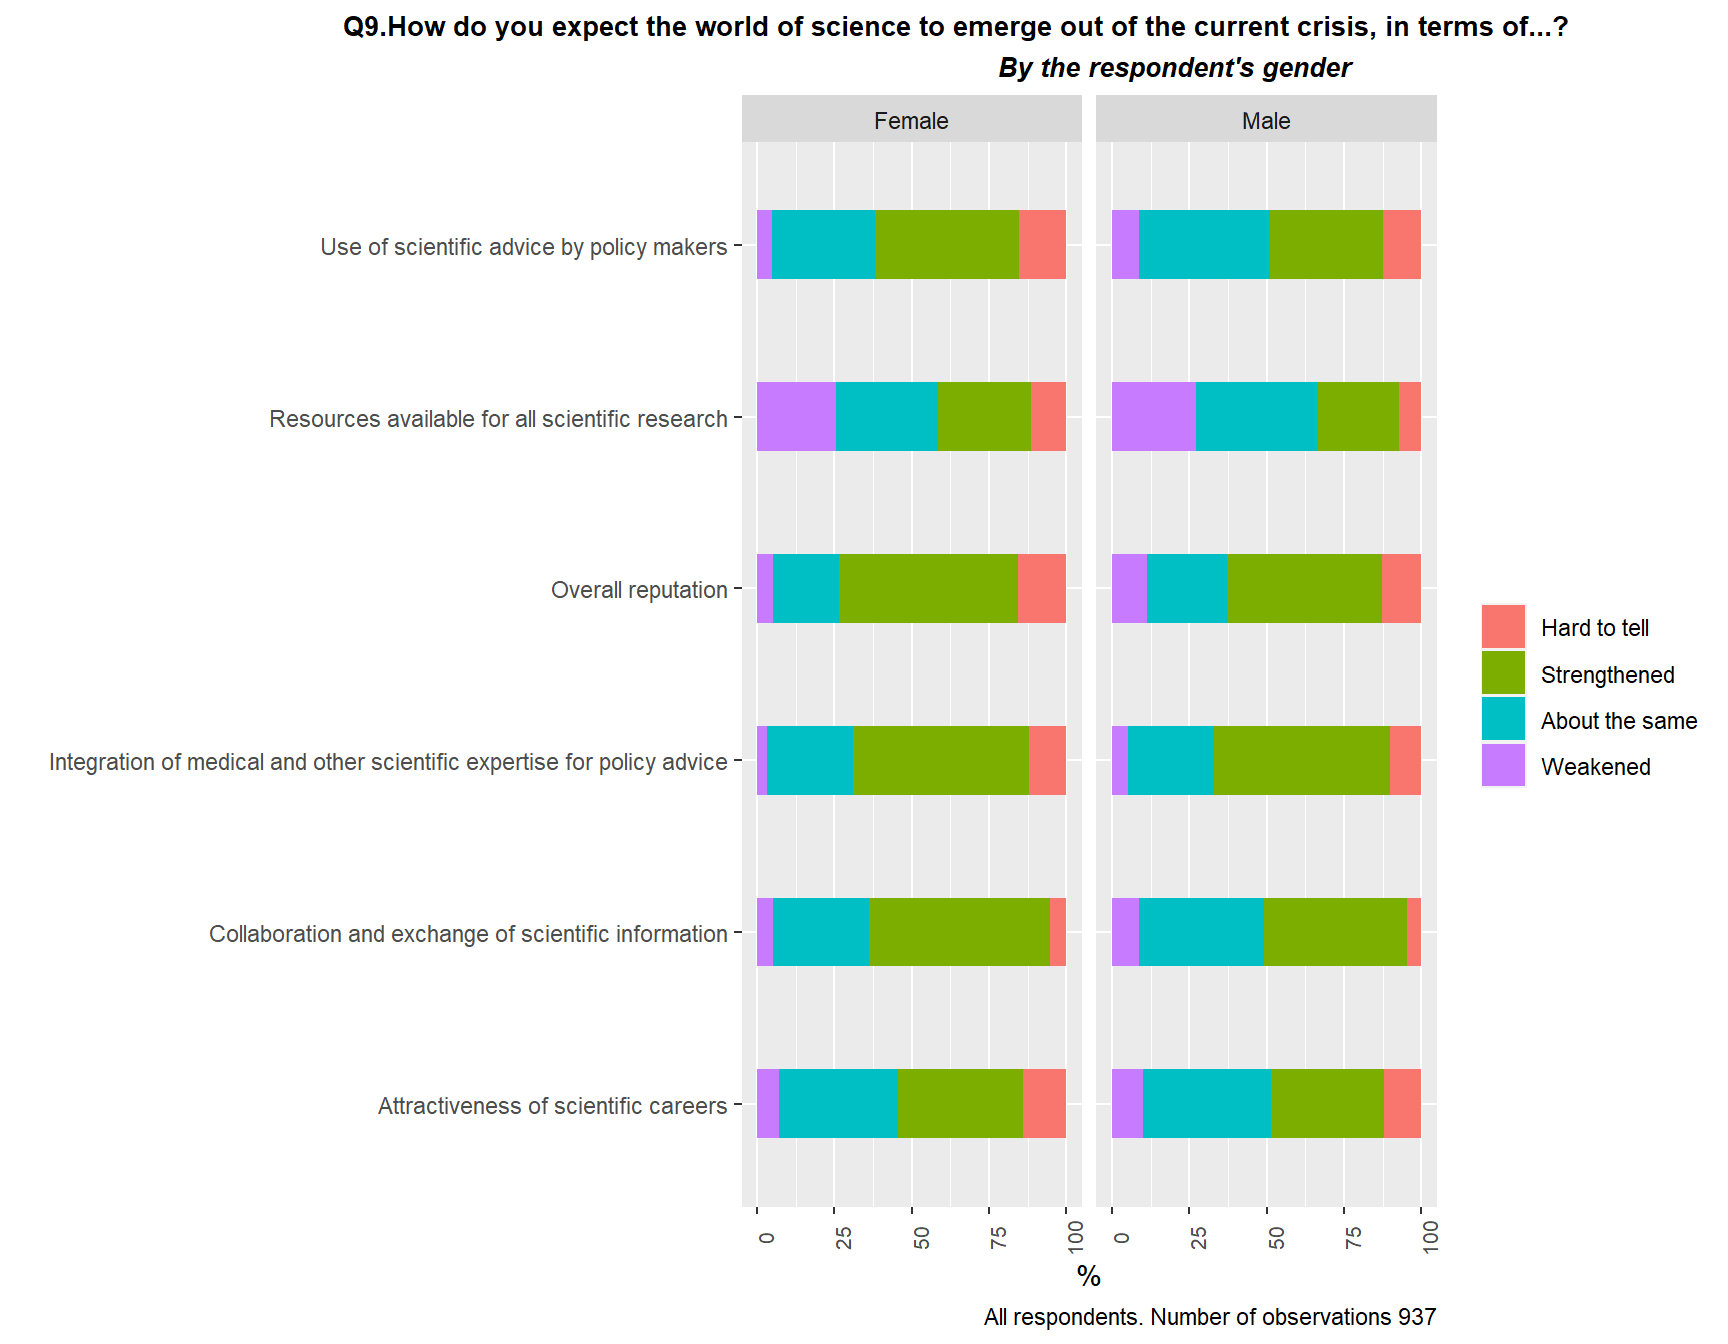
\includegraphics{V:/Bello_M/BACKUP/Science Barometer/Git/2020flashsciencecovid/docs/index_files/figure-latex/plot_corecharts9-1.pdf}
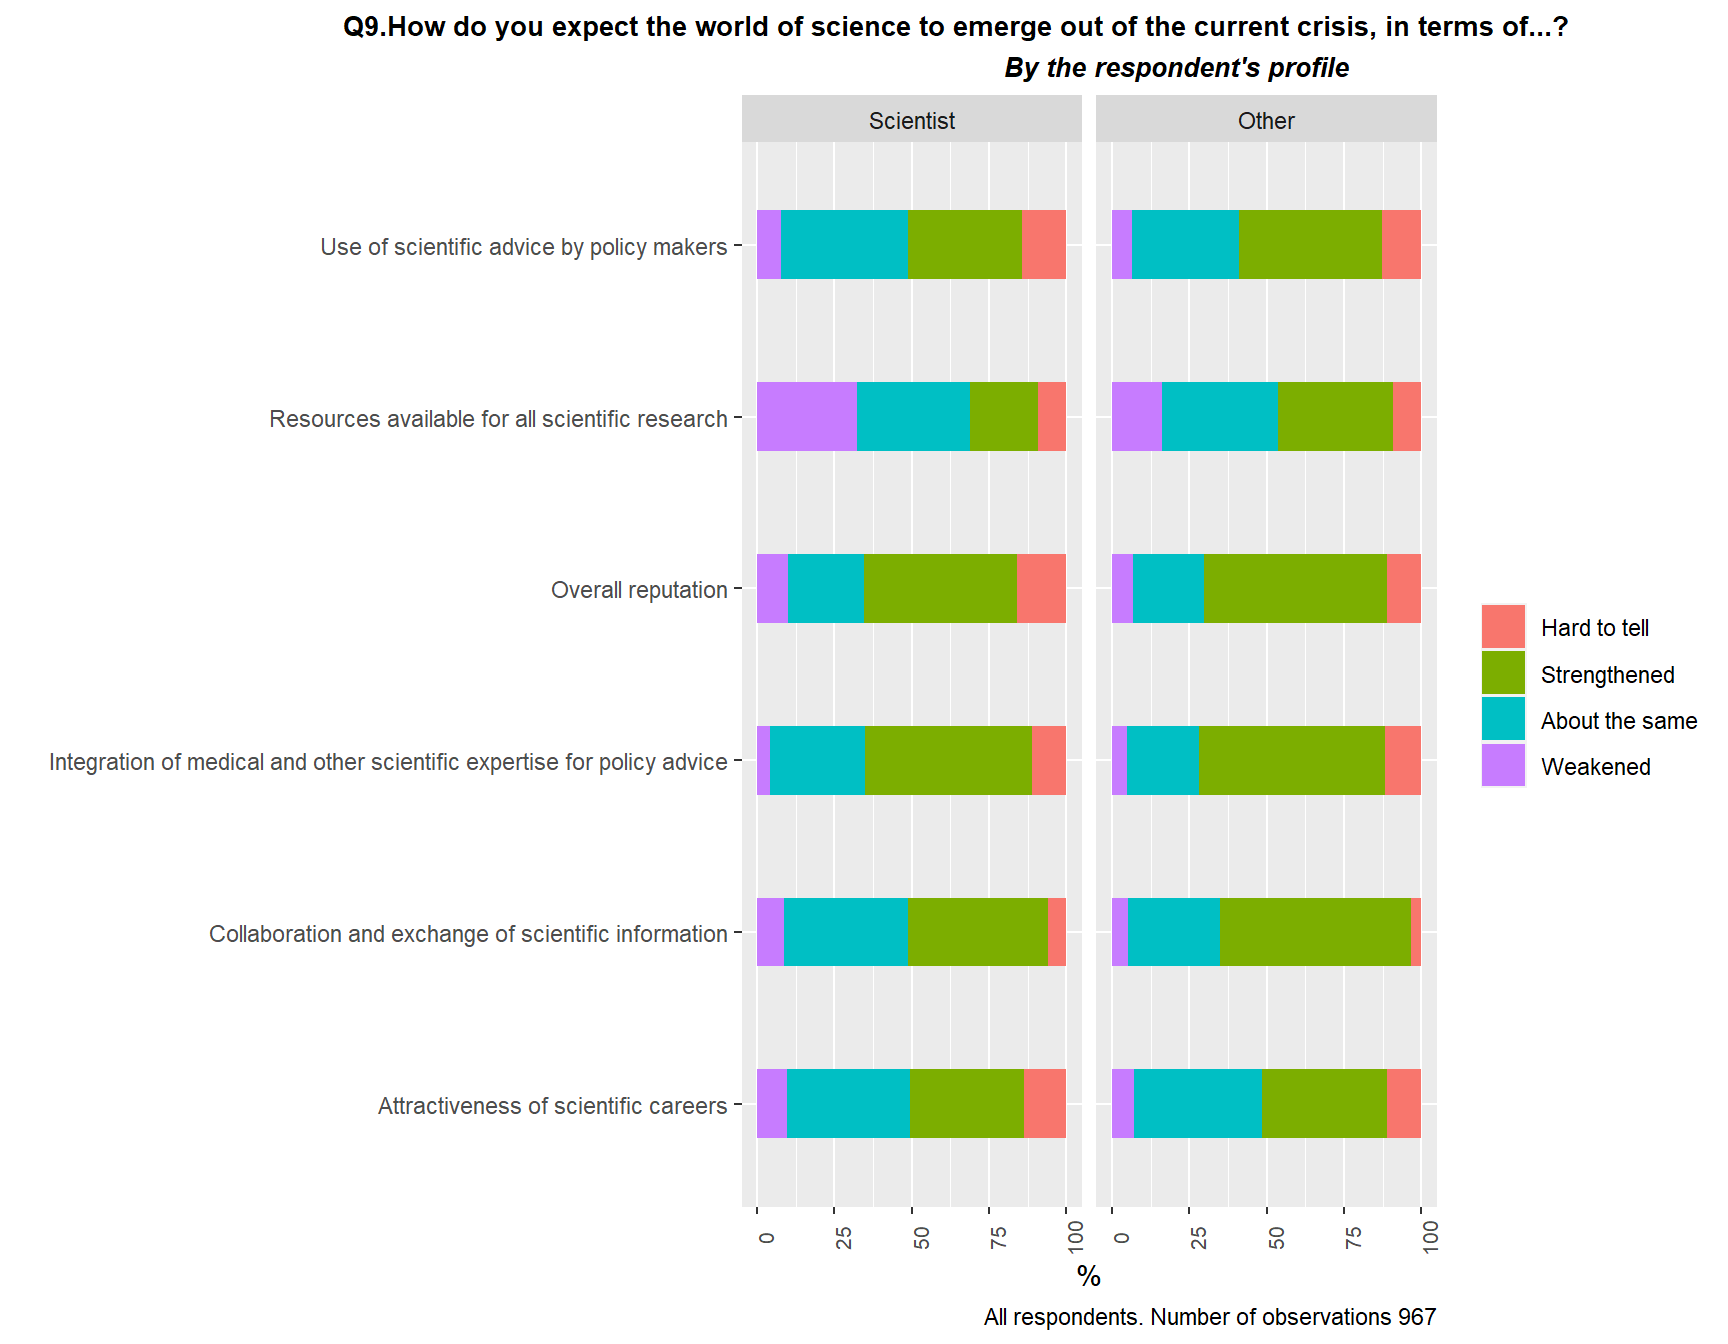
\includegraphics{V:/Bello_M/BACKUP/Science Barometer/Git/2020flashsciencecovid/docs/index_files/figure-latex/plot_corecharts9-2.pdf}

\hypertarget{next-steps-for-the-science-covid-flash-survey}{%
\subsection{\texorpdfstring{\textbf{Next steps for the Science-COVID
flash
survey}}{Next steps for the Science-COVID flash survey}}\label{next-steps-for-the-science-covid-flash-survey}}

The results of this experimental flash/pulse study may inform OECD work
on policy responses to the COVID-19 crisis. The survey will remain open
on the following link while the current questions remain relevant:
\url{https://survey.oecd.org/index.php?r=survey/index\&sid=176928\&lang=en}

As participation grows, additional data breakdowns will be available and
results may be also mapped over time. As circumstances change, the OECD
will consider the relevance of updating the questionnaire with questions
that allow to track specific items of policy and social interest. The
anonymous microdata for this study will be made available for secondary
research purposes.

\textbf{You can help improve the robustness of these results by sharing
this document/link with your network. For further information, please
contact: issa@oecd.org }

\hypertarget{detailed-results}{%
\subsection{\texorpdfstring{\textbf{Detailed
results}}{Detailed results}}\label{detailed-results}}

\hypertarget{respondent-profile}{%
\section{\texorpdfstring{\emph{Respondent
profile}}{Respondent profile}}\label{respondent-profile}}

North and South America is the most represented geographical region in
this study (64\% of respondents) followed by Europe (28\%), Asia and
Oceania (7\%), and Africa (1\%). The majority of respondents are aged
between 35 and 55 years old. Men slightly outnumber women in terms of
participation.

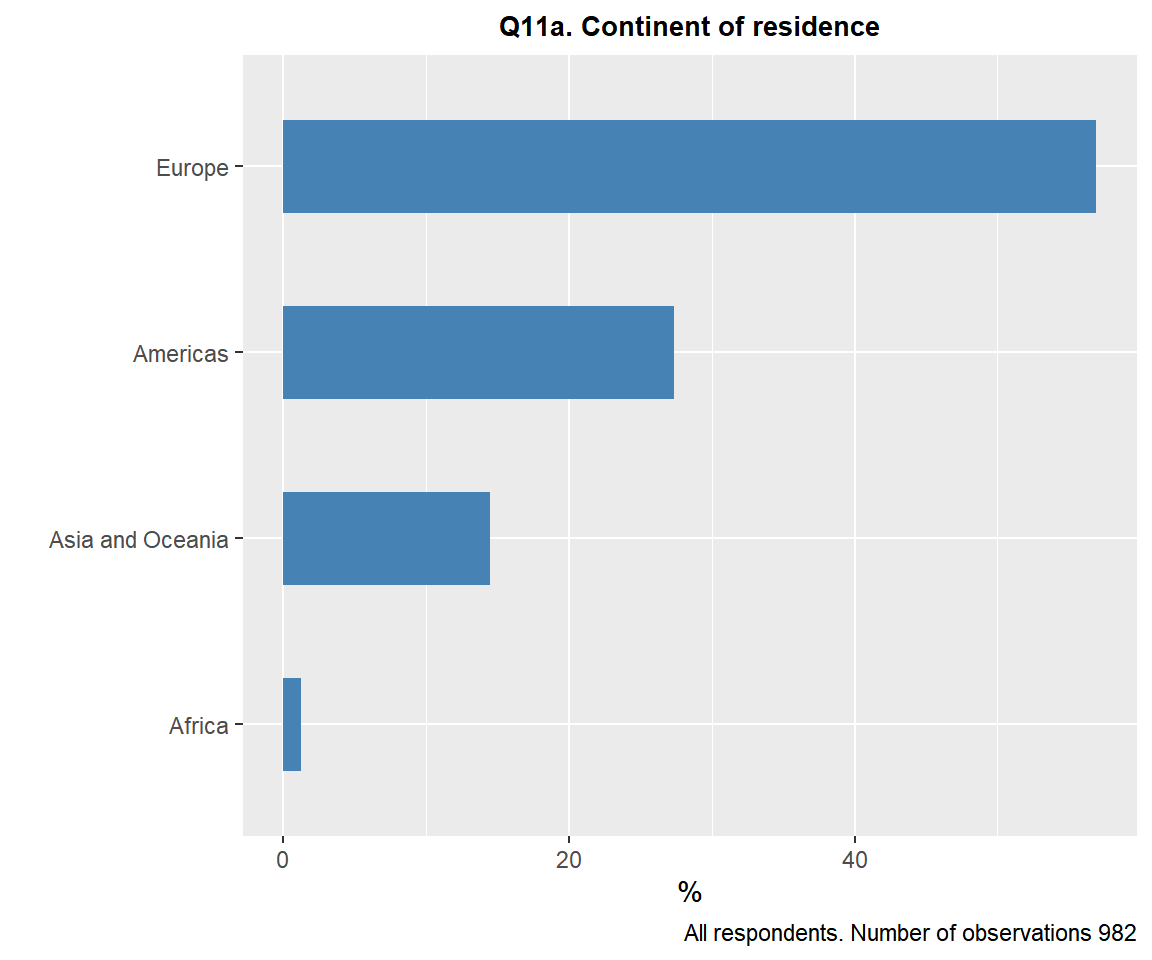
\includegraphics{V:/Bello_M/BACKUP/Science Barometer/Git/2020flashsciencecovid/docs/index_files/figure-latex/plot_respcharts1-1.pdf}
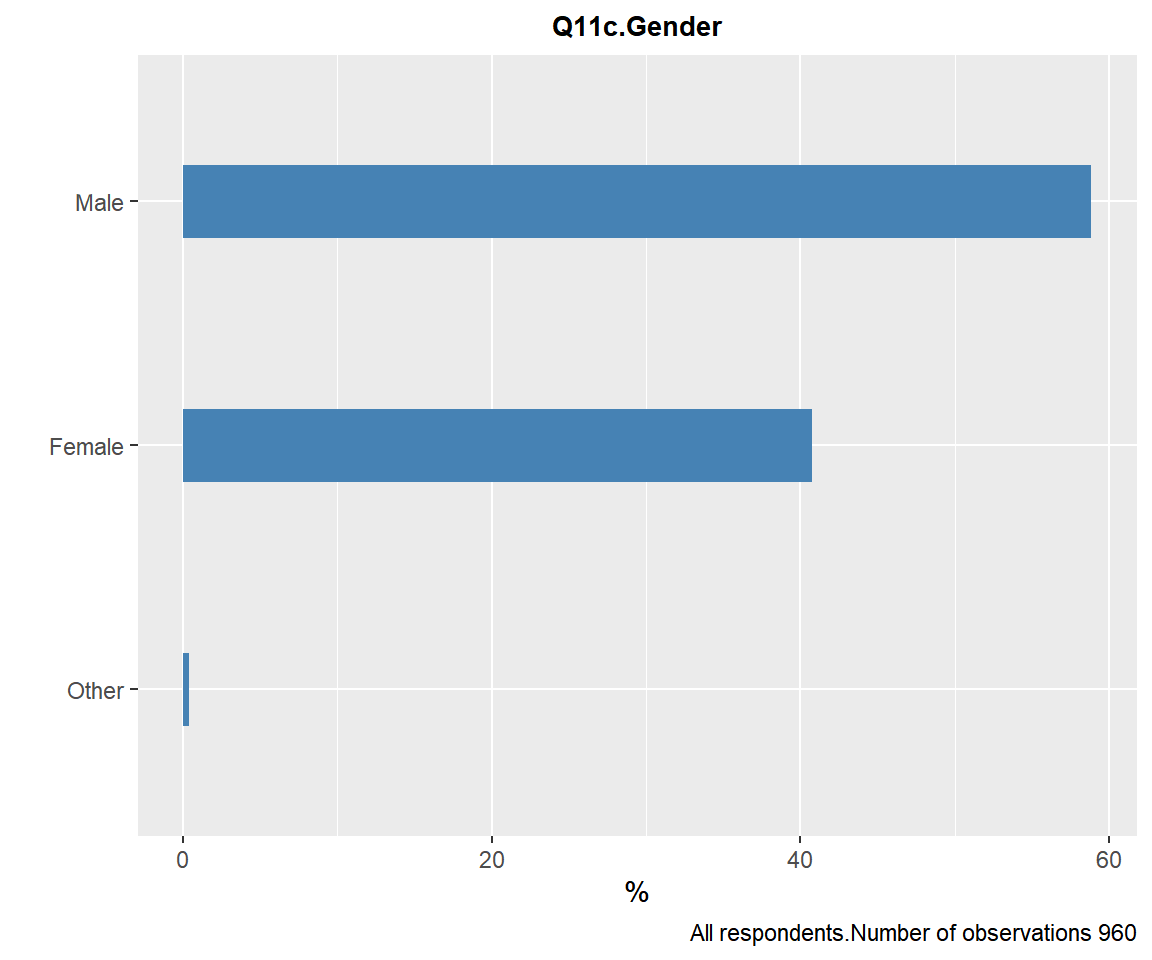
\includegraphics{V:/Bello_M/BACKUP/Science Barometer/Git/2020flashsciencecovid/docs/index_files/figure-latex/plot_respcharts1-2.pdf}
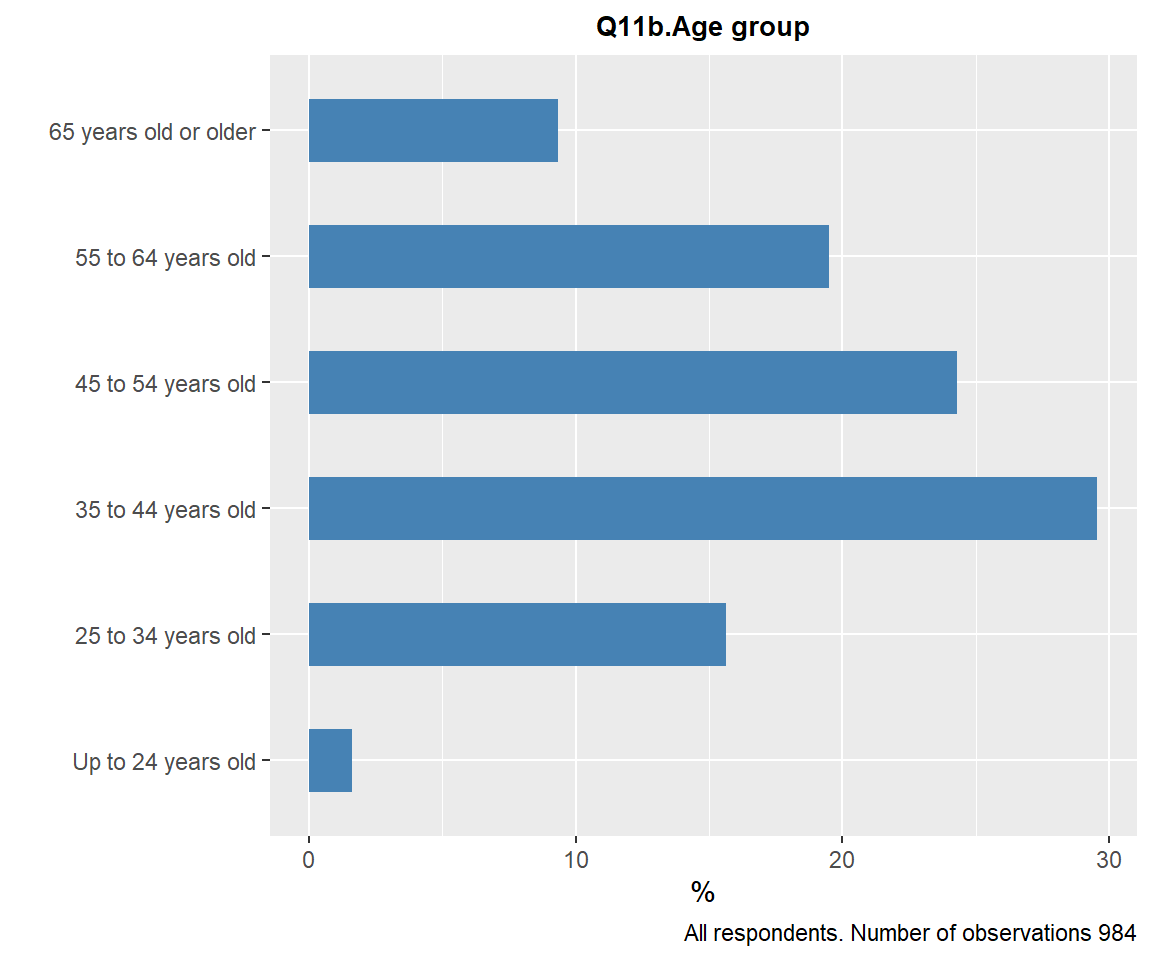
\includegraphics{V:/Bello_M/BACKUP/Science Barometer/Git/2020flashsciencecovid/docs/index_files/figure-latex/plot_respcharts1-3.pdf}
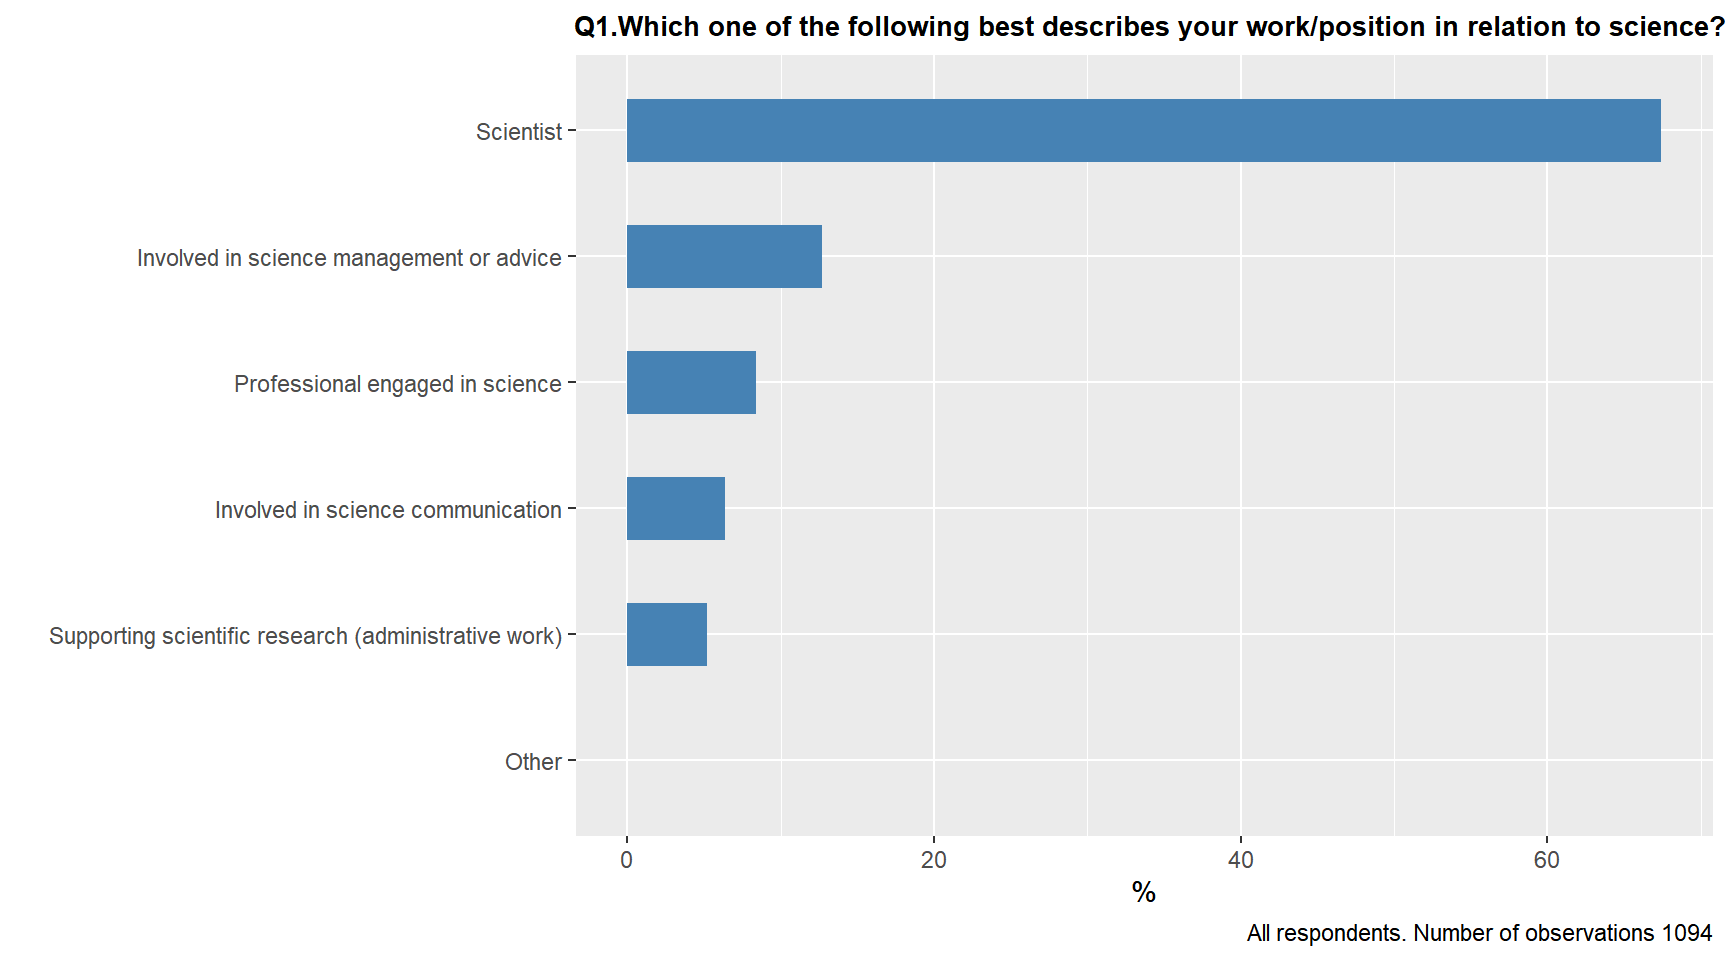
\includegraphics{V:/Bello_M/BACKUP/Science Barometer/Git/2020flashsciencecovid/docs/index_files/figure-latex/plot_corecharts2-1.pdf}

\hypertarget{current-situation}{%
\section{\texorpdfstring{\emph{Current
situation}}{Current situation}}\label{current-situation}}

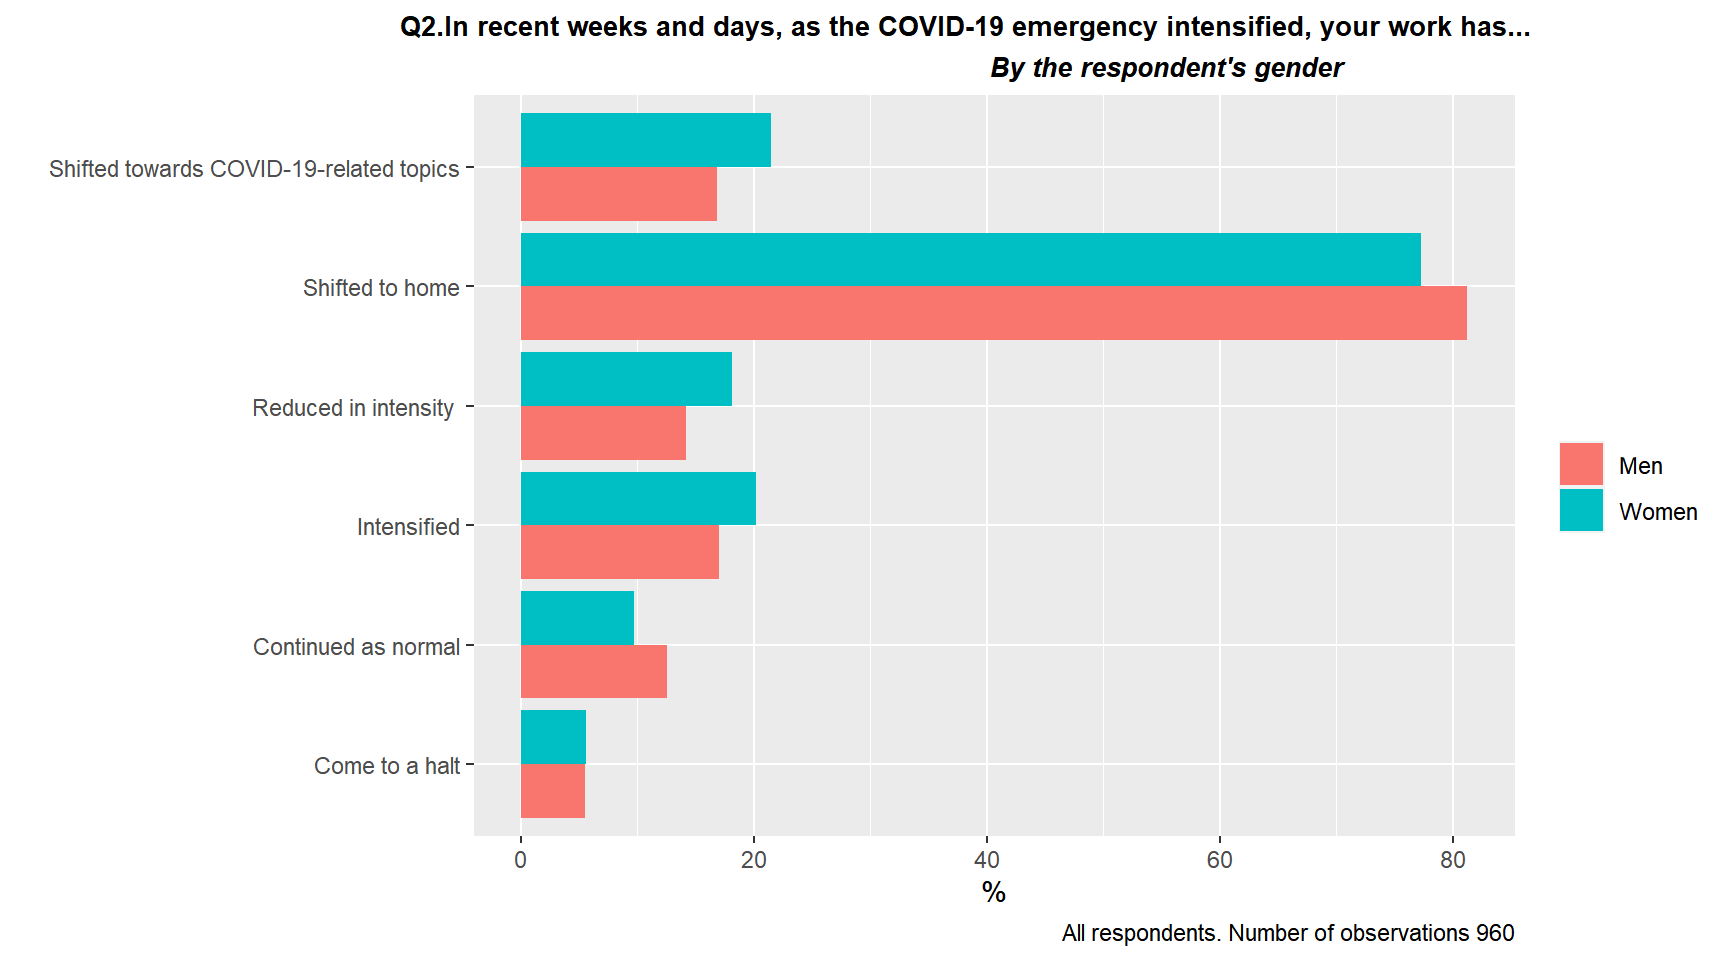
\includegraphics{V:/Bello_M/BACKUP/Science Barometer/Git/2020flashsciencecovid/docs/index_files/figure-latex/plot_corecharts3-1.pdf}
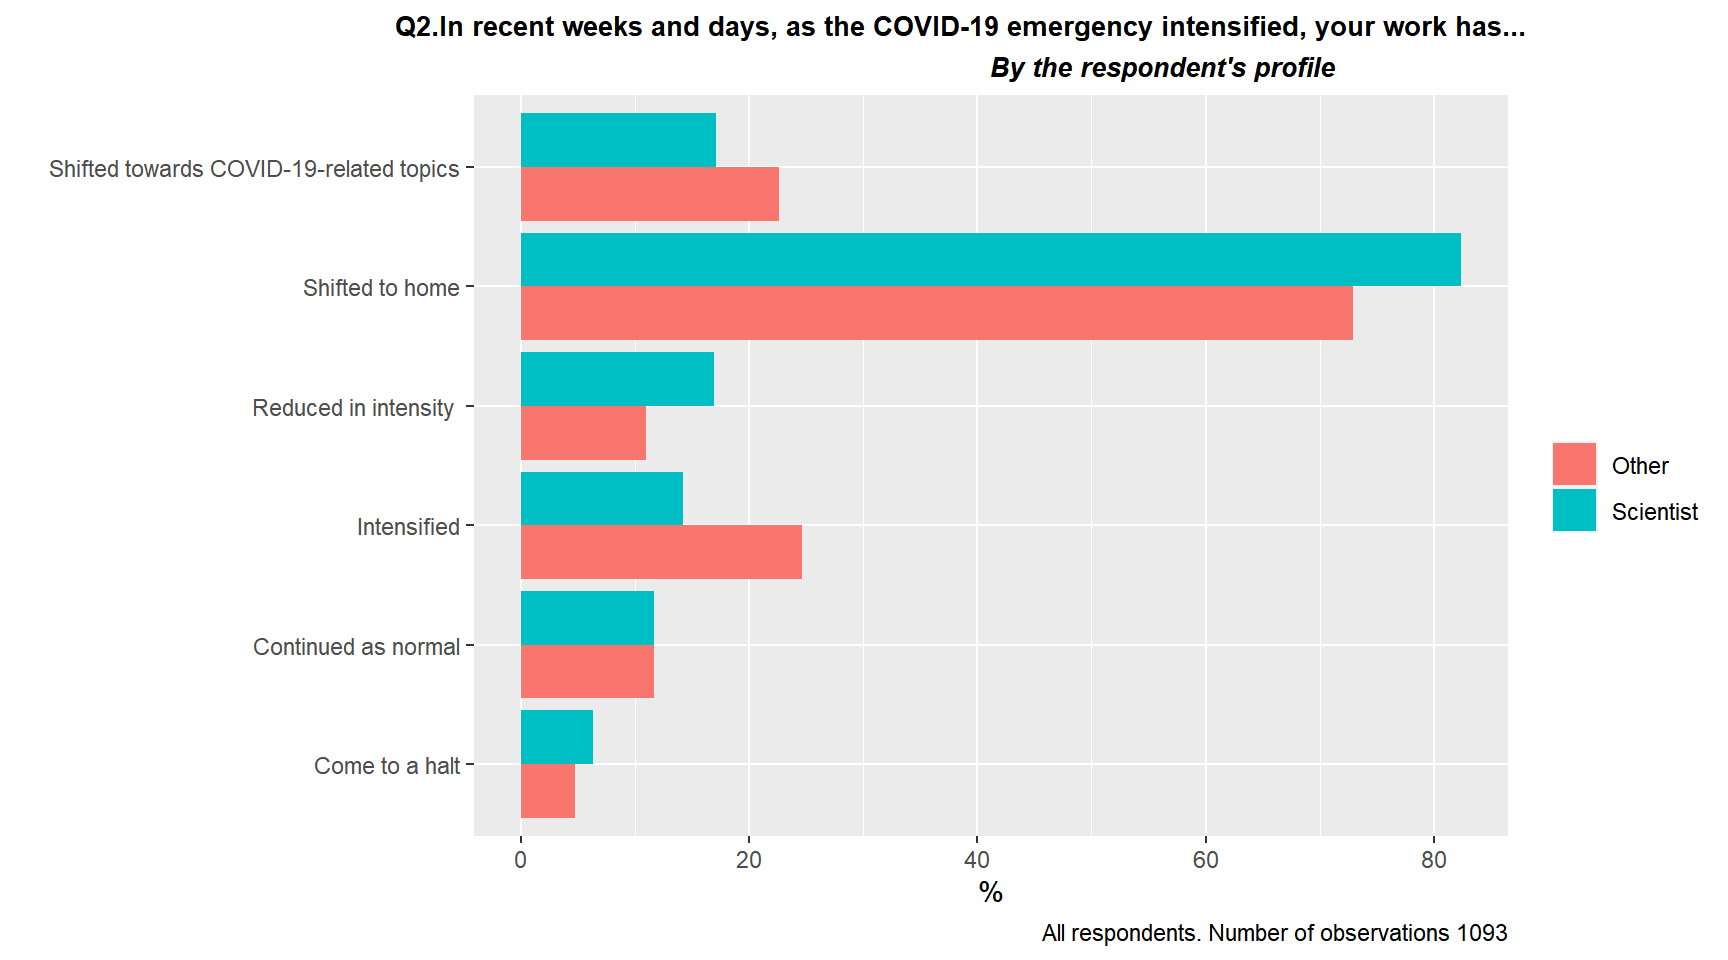
\includegraphics{V:/Bello_M/BACKUP/Science Barometer/Git/2020flashsciencecovid/docs/index_files/figure-latex/plot_corecharts3-2.pdf}

\hypertarget{impacts-on-current-research-scientists}{%
\section{\texorpdfstring{\emph{Impacts on current research
(scientists)}}{Impacts on current research (scientists)}}\label{impacts-on-current-research-scientists}}

Over 60\% of the individuals that participated in this study are
scientists. The majority of them are specialised in biochemistry,
genetics and molecular biology, agricultural and biological sciences,
science policy, and arts and humanities.

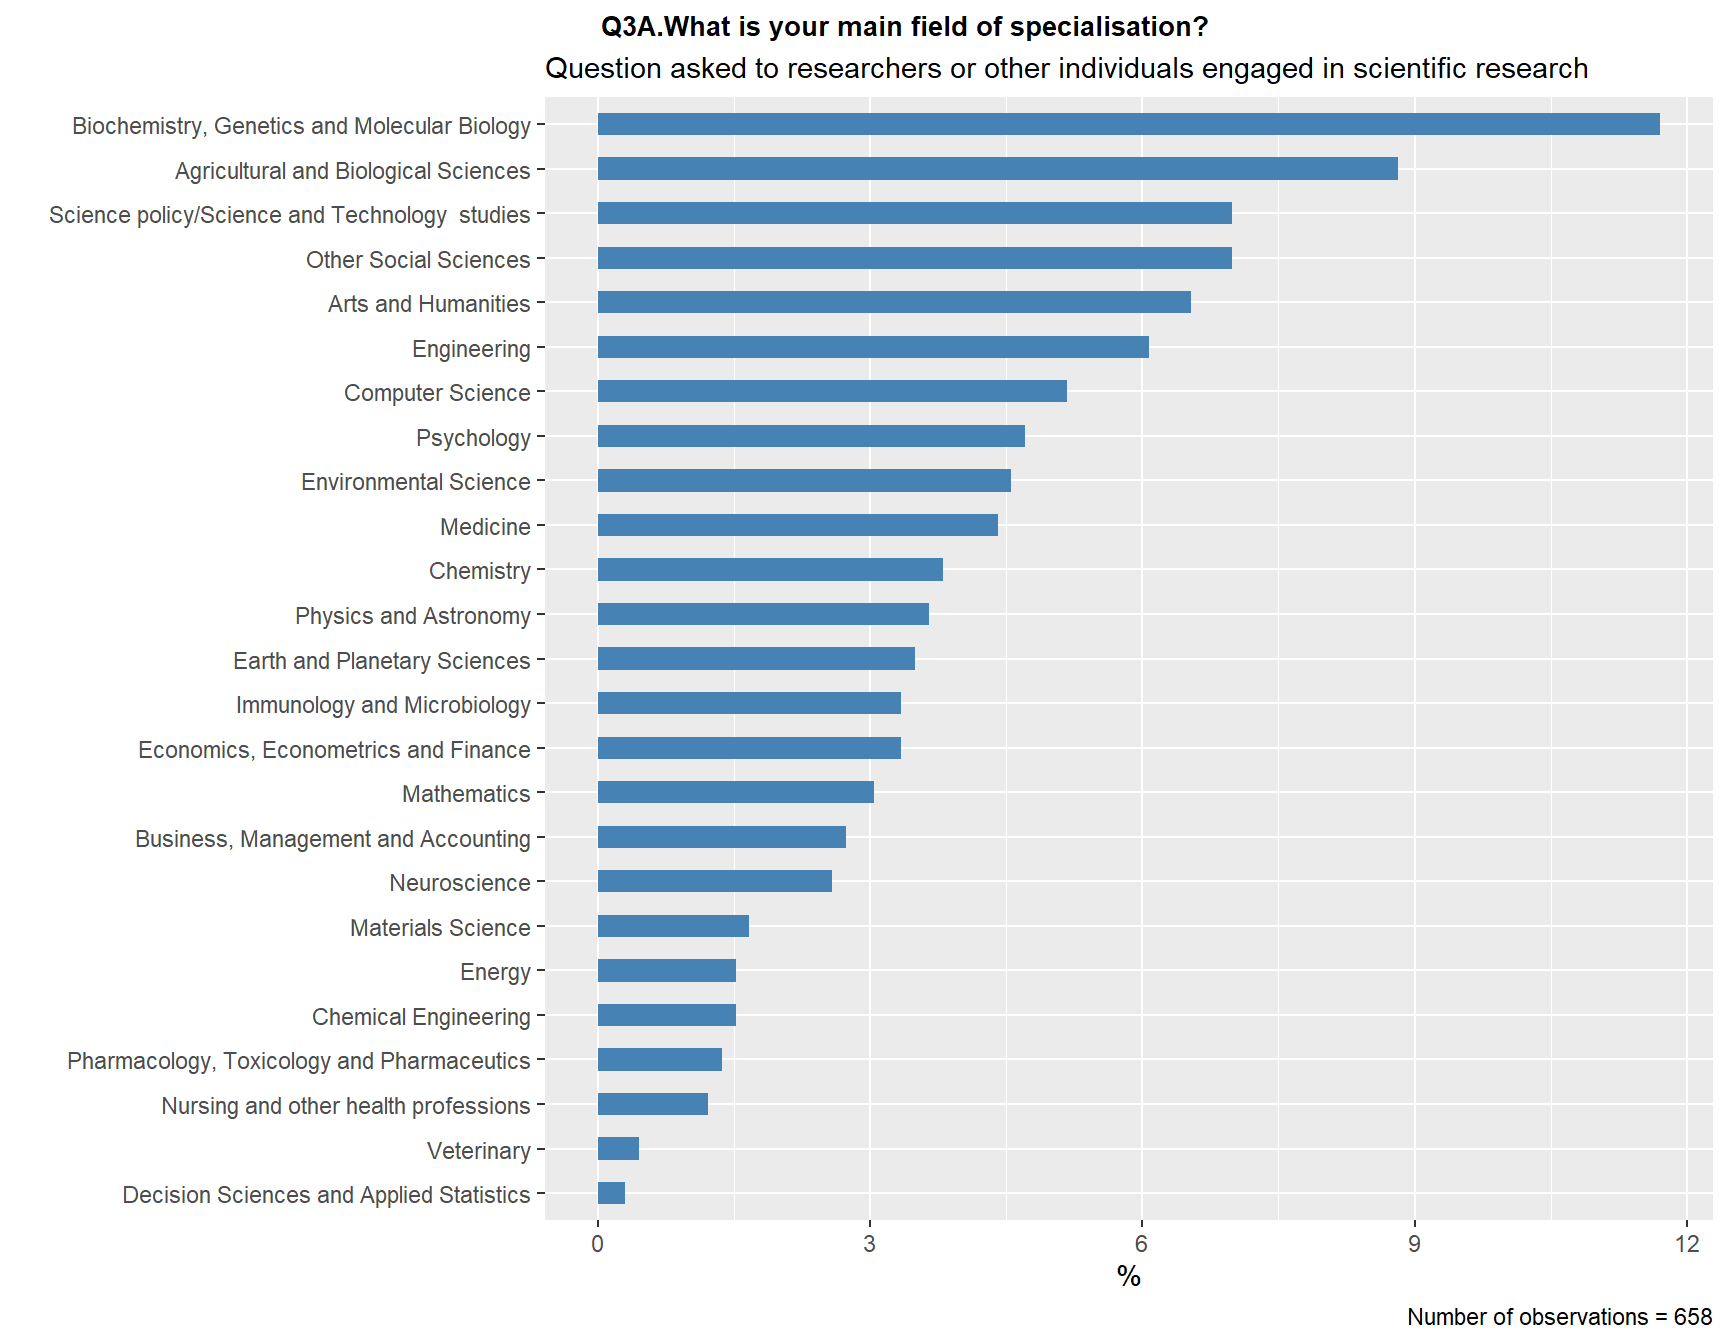
\includegraphics{V:/Bello_M/BACKUP/Science Barometer/Git/2020flashsciencecovid/docs/index_files/figure-latex/plot_corecharts4-1.pdf}
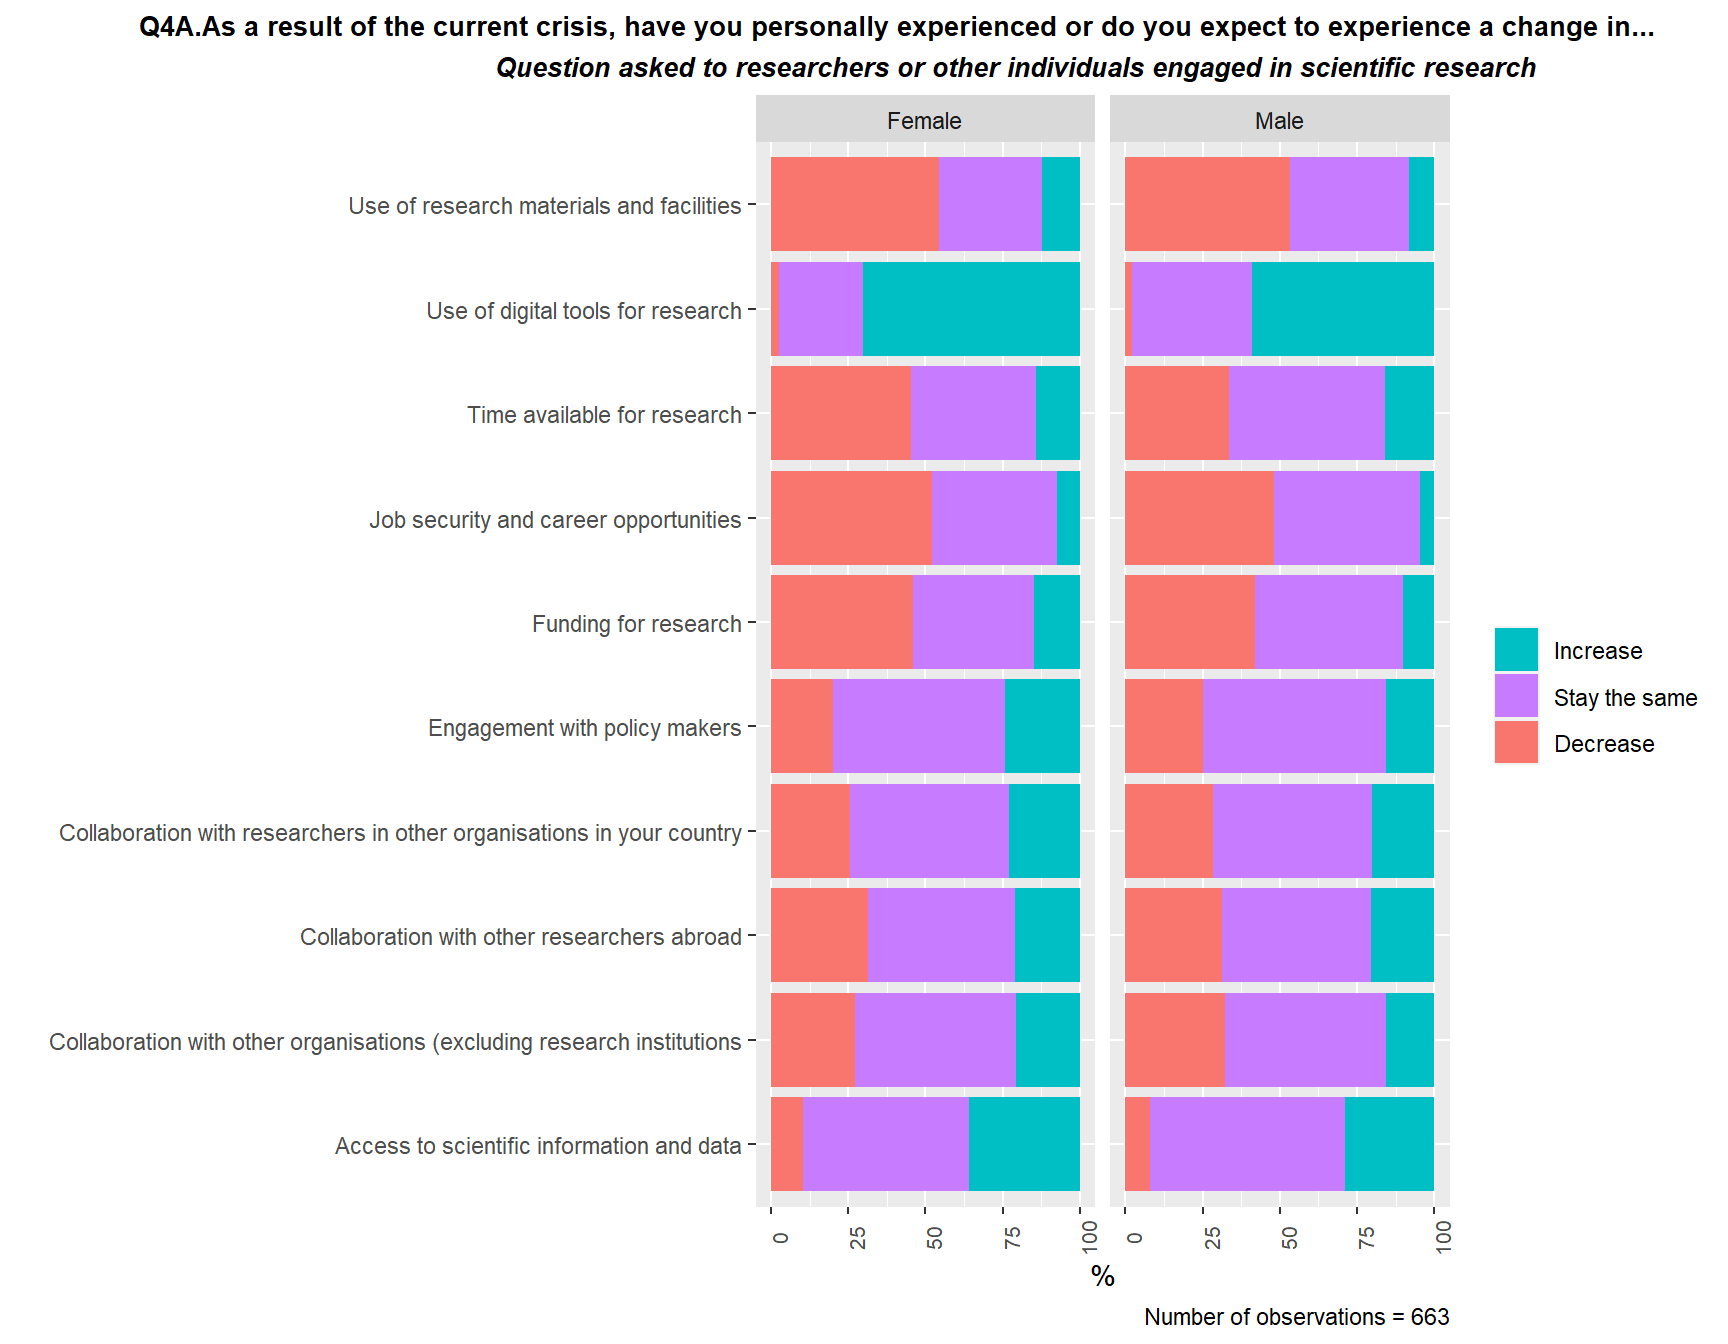
\includegraphics{V:/Bello_M/BACKUP/Science Barometer/Git/2020flashsciencecovid/docs/index_files/figure-latex/plot_corecharts4-2.pdf}
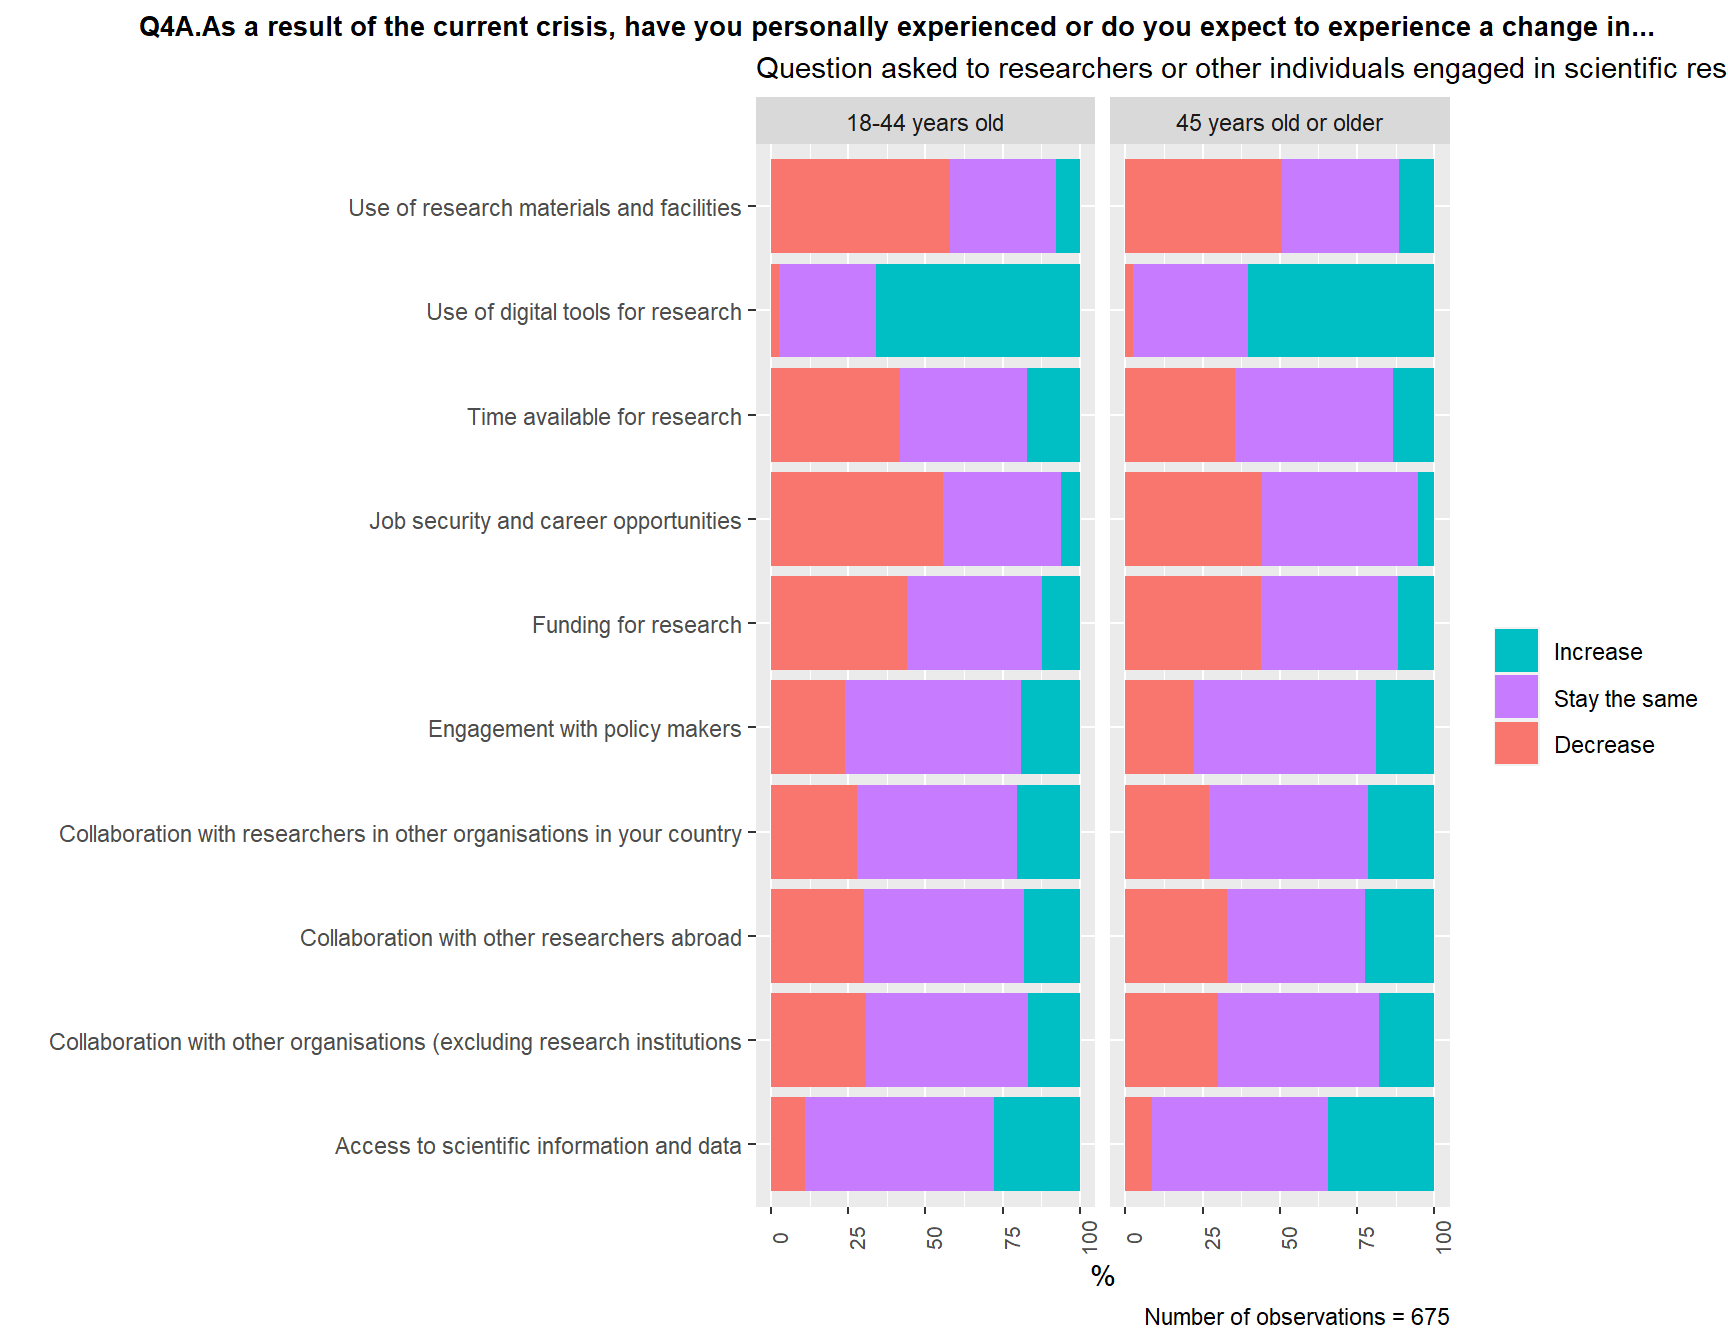
\includegraphics{V:/Bello_M/BACKUP/Science Barometer/Git/2020flashsciencecovid/docs/index_files/figure-latex/plot_corecharts4-3.pdf}

\hypertarget{assessment-of-the-use-of-science-in-policy-making-policy-makersadvisorscommunicators}{%
\section{\texorpdfstring{\emph{Assessment of the use of science in
policy making (policy
makers/advisors/communicators)}}{Assessment of the use of science in policy making (policy makers/advisors/communicators)}}\label{assessment-of-the-use-of-science-in-policy-making-policy-makersadvisorscommunicators}}

Decision/policy advisors, makers or communicators that responded to the
survey source information for their work mainly from science
policy/science and technology studies, energy and environmental
sciences, biochemistry, genetics and molecular biology, and social
sciences. Among this group of respondents, policy analysts or advisors
are those that regularly engage with scientists and researchers the
most, followed by the science communicators.

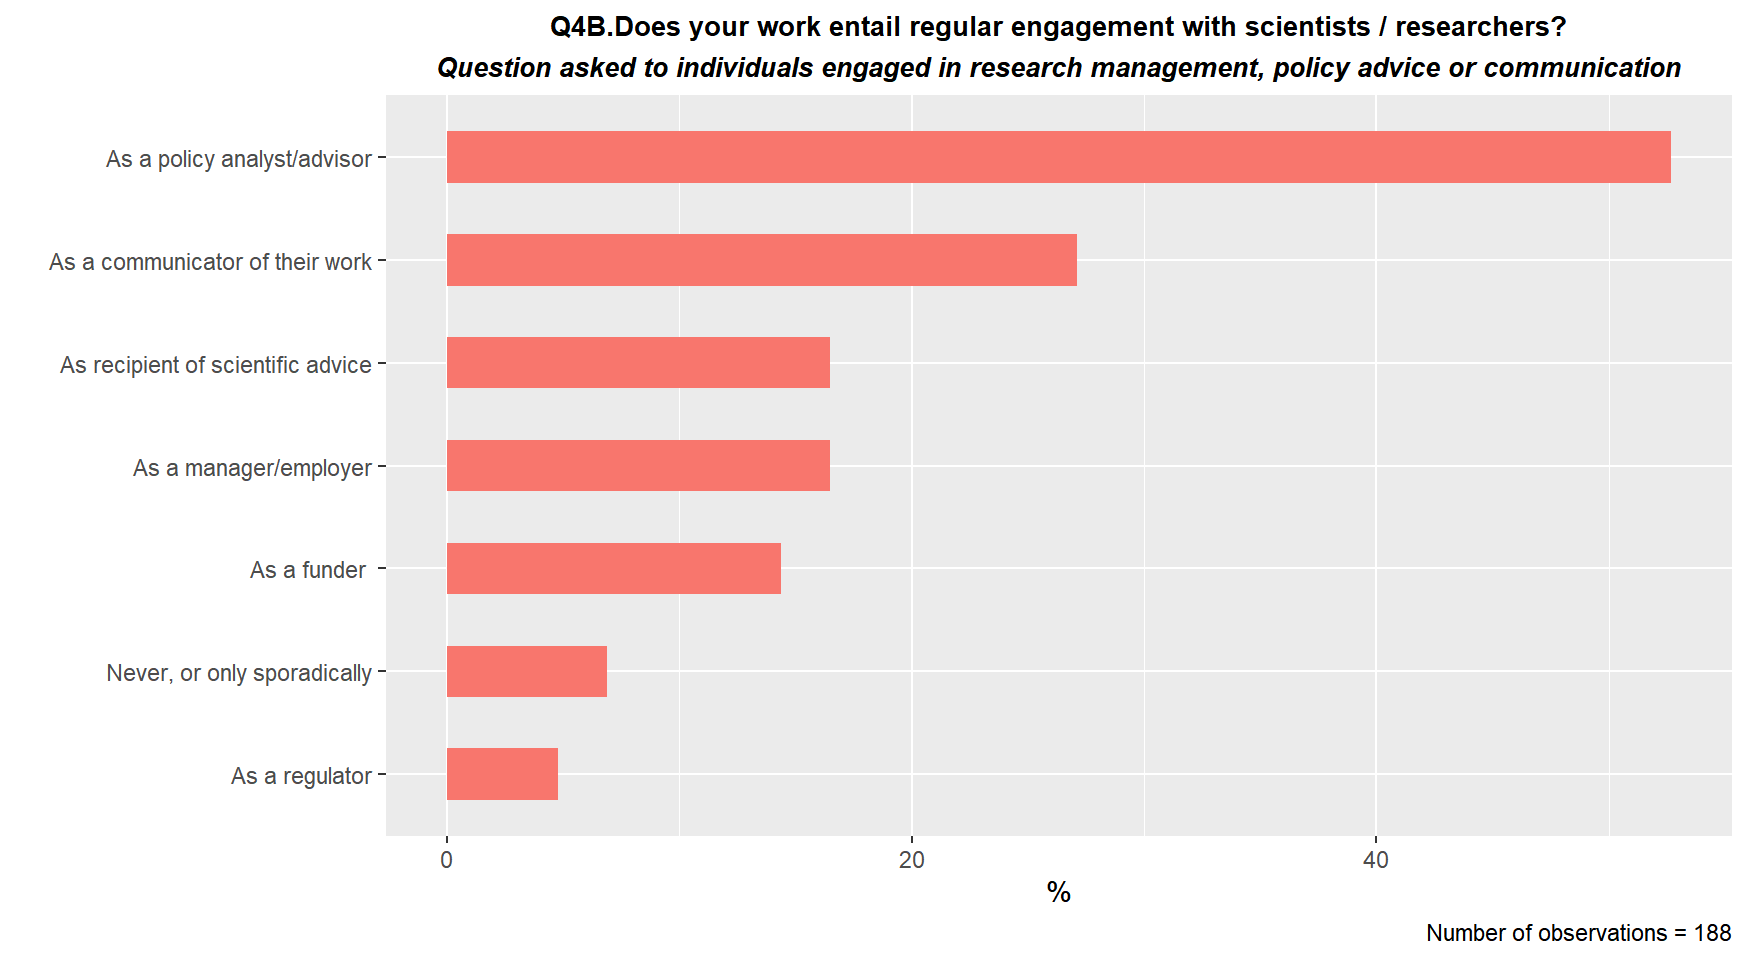
\includegraphics{V:/Bello_M/BACKUP/Science Barometer/Git/2020flashsciencecovid/docs/index_files/figure-latex/plot_corecharts5-1.pdf}
\includegraphics{V:/Bello_M/BACKUP/Science Barometer/Git/2020flashsciencecovid/docs/index_files/figure-latex/plot_corecharts6-1.pdf}

\hypertarget{trusted-sources-of-information}{%
\section{\texorpdfstring{\emph{Trusted sources of
information}}{Trusted sources of information}}\label{trusted-sources-of-information}}

\includegraphics{V:/Bello_M/BACKUP/Science Barometer/Git/2020flashsciencecovid/docs/index_files/figure-latex/plot_corecharts7-1.pdf}
\includegraphics{V:/Bello_M/BACKUP/Science Barometer/Git/2020flashsciencecovid/docs/index_files/figure-latex/plot_corecharts7-2.pdf}

\hypertarget{trust-in-decision-makers}{%
\section{\texorpdfstring{\emph{Trust in decision
makers}}{Trust in decision makers}}\label{trust-in-decision-makers}}

\includegraphics{V:/Bello_M/BACKUP/Science Barometer/Git/2020flashsciencecovid/docs/index_files/figure-latex/plot_corecharts8-1.pdf}
\includegraphics{V:/Bello_M/BACKUP/Science Barometer/Git/2020flashsciencecovid/docs/index_files/figure-latex/plot_corecharts8-2.pdf}
\includegraphics{V:/Bello_M/BACKUP/Science Barometer/Git/2020flashsciencecovid/docs/index_files/figure-latex/plot_corecharts8-3.pdf}

\hypertarget{participate-in-the-survey}{%
\section{Participate in the survey}\label{participate-in-the-survey}}

Contact us

Click here to access the OECD Terms and Conditions

\end{document}
